\begin{figure}[b]
\centerline{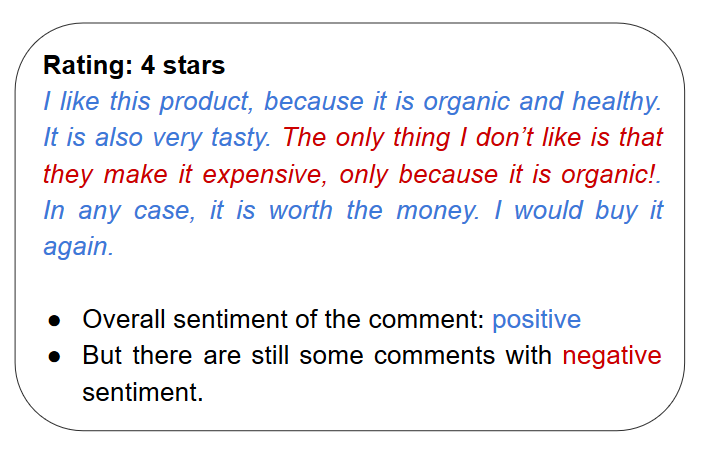
\includegraphics[scale=.5]{images/comment_example.png}}
\caption{Example of a positive comment with negative sentences.}
\label{comment_example}
\end{figure}

Today, the  long-term  goal  of  developing  sustainable  food systems is considered a high priority by several intergovernmental  organizations \cite{Mie2017}. This has lead to developments in modern organic food production, largely driven by the ideal of sustainability and environmental concern \cite{healthyNutritiousFood}.\\
In order to create successful strategies to promote production and consumption of organic food, it is necessary to understand the opinions of the general public regarding organic products. For this, it is useful to understand the sentiment of comments about organic food in a sentence level. This is illustrated in Figure \ref{comment_example} showing that even though the overall sentiment of the comment is positive, there are sentences that are clearly negative. This would be ignored if we analyzed only the sentiment of the comment, and not the sentiment of each sentence.\\
In addition to the above, Web 2.0 has led to the emergence of blogs, forums, and online social networks that enable users to discuss any topic and share their opinions about it \cite{Dang_2020}. For this reason, coarse-grained document-level annotations are relatively easy to obtain. Despite this, the acquisition of  sentence-  or  phrase-level  sentiment  labels  remains  a  laborious  and  expensive endeavor even tough they are relevant to various opinion mining applications \cite{angelidis2017multiple}, including sentiment analysis.\\
For all these reasons, a model that allows us to understand sentiment in a sentence level for the organic food domain based on comments is important.\\
In this paper, we will explore the use of Multi-Instance Learning Networks, which only require document-level supervision and learns to introspectively judge the sentiment  of  constituent  segments \cite{angelidis2017multiple} for sentence-level sentiment analysis in the context of organic products. For this, we will use use data from Amazon reviews in English and German, together with a dataset that contains annotated sentences from Quora about organic products.\\
Also, we will explore the effects of using transfer learning together with Multi-Instance Learning Networks and compare the results obtained by using different initial sentence embeddings.\\
Finally, we will investigate the use of Multi-Instance Learning Networks in cross-lingual tasks for English and German data. \\
